\chapter{Philosophy}
\label{ch:philosophy}

\begin{chapquote}{Lewis Carroll, \textit{Alice in Wonderland}}
The mouse looked at her rather inquisitively, and seemed to her to wink with one
of its little eyes, but it said nothing.
\end{chapquote}

\newthought{Looking at Bitcoin} superficially, one might conclude that it is slow, wasteful,
unnecessarily redundant, and overly paranoid. Looking at Bitcoin inquisitively,
one might find out that things are not as they seem at first glance.

Bitcoin has a way of taking your assumptions and turning them on their heads.
After a while, just when you were about to get comfortable again, Bitcoin will
smash through the wall like a bull in a china shop and shatter your assumptions
once more.

\begin{figure}[ht!]
\centering
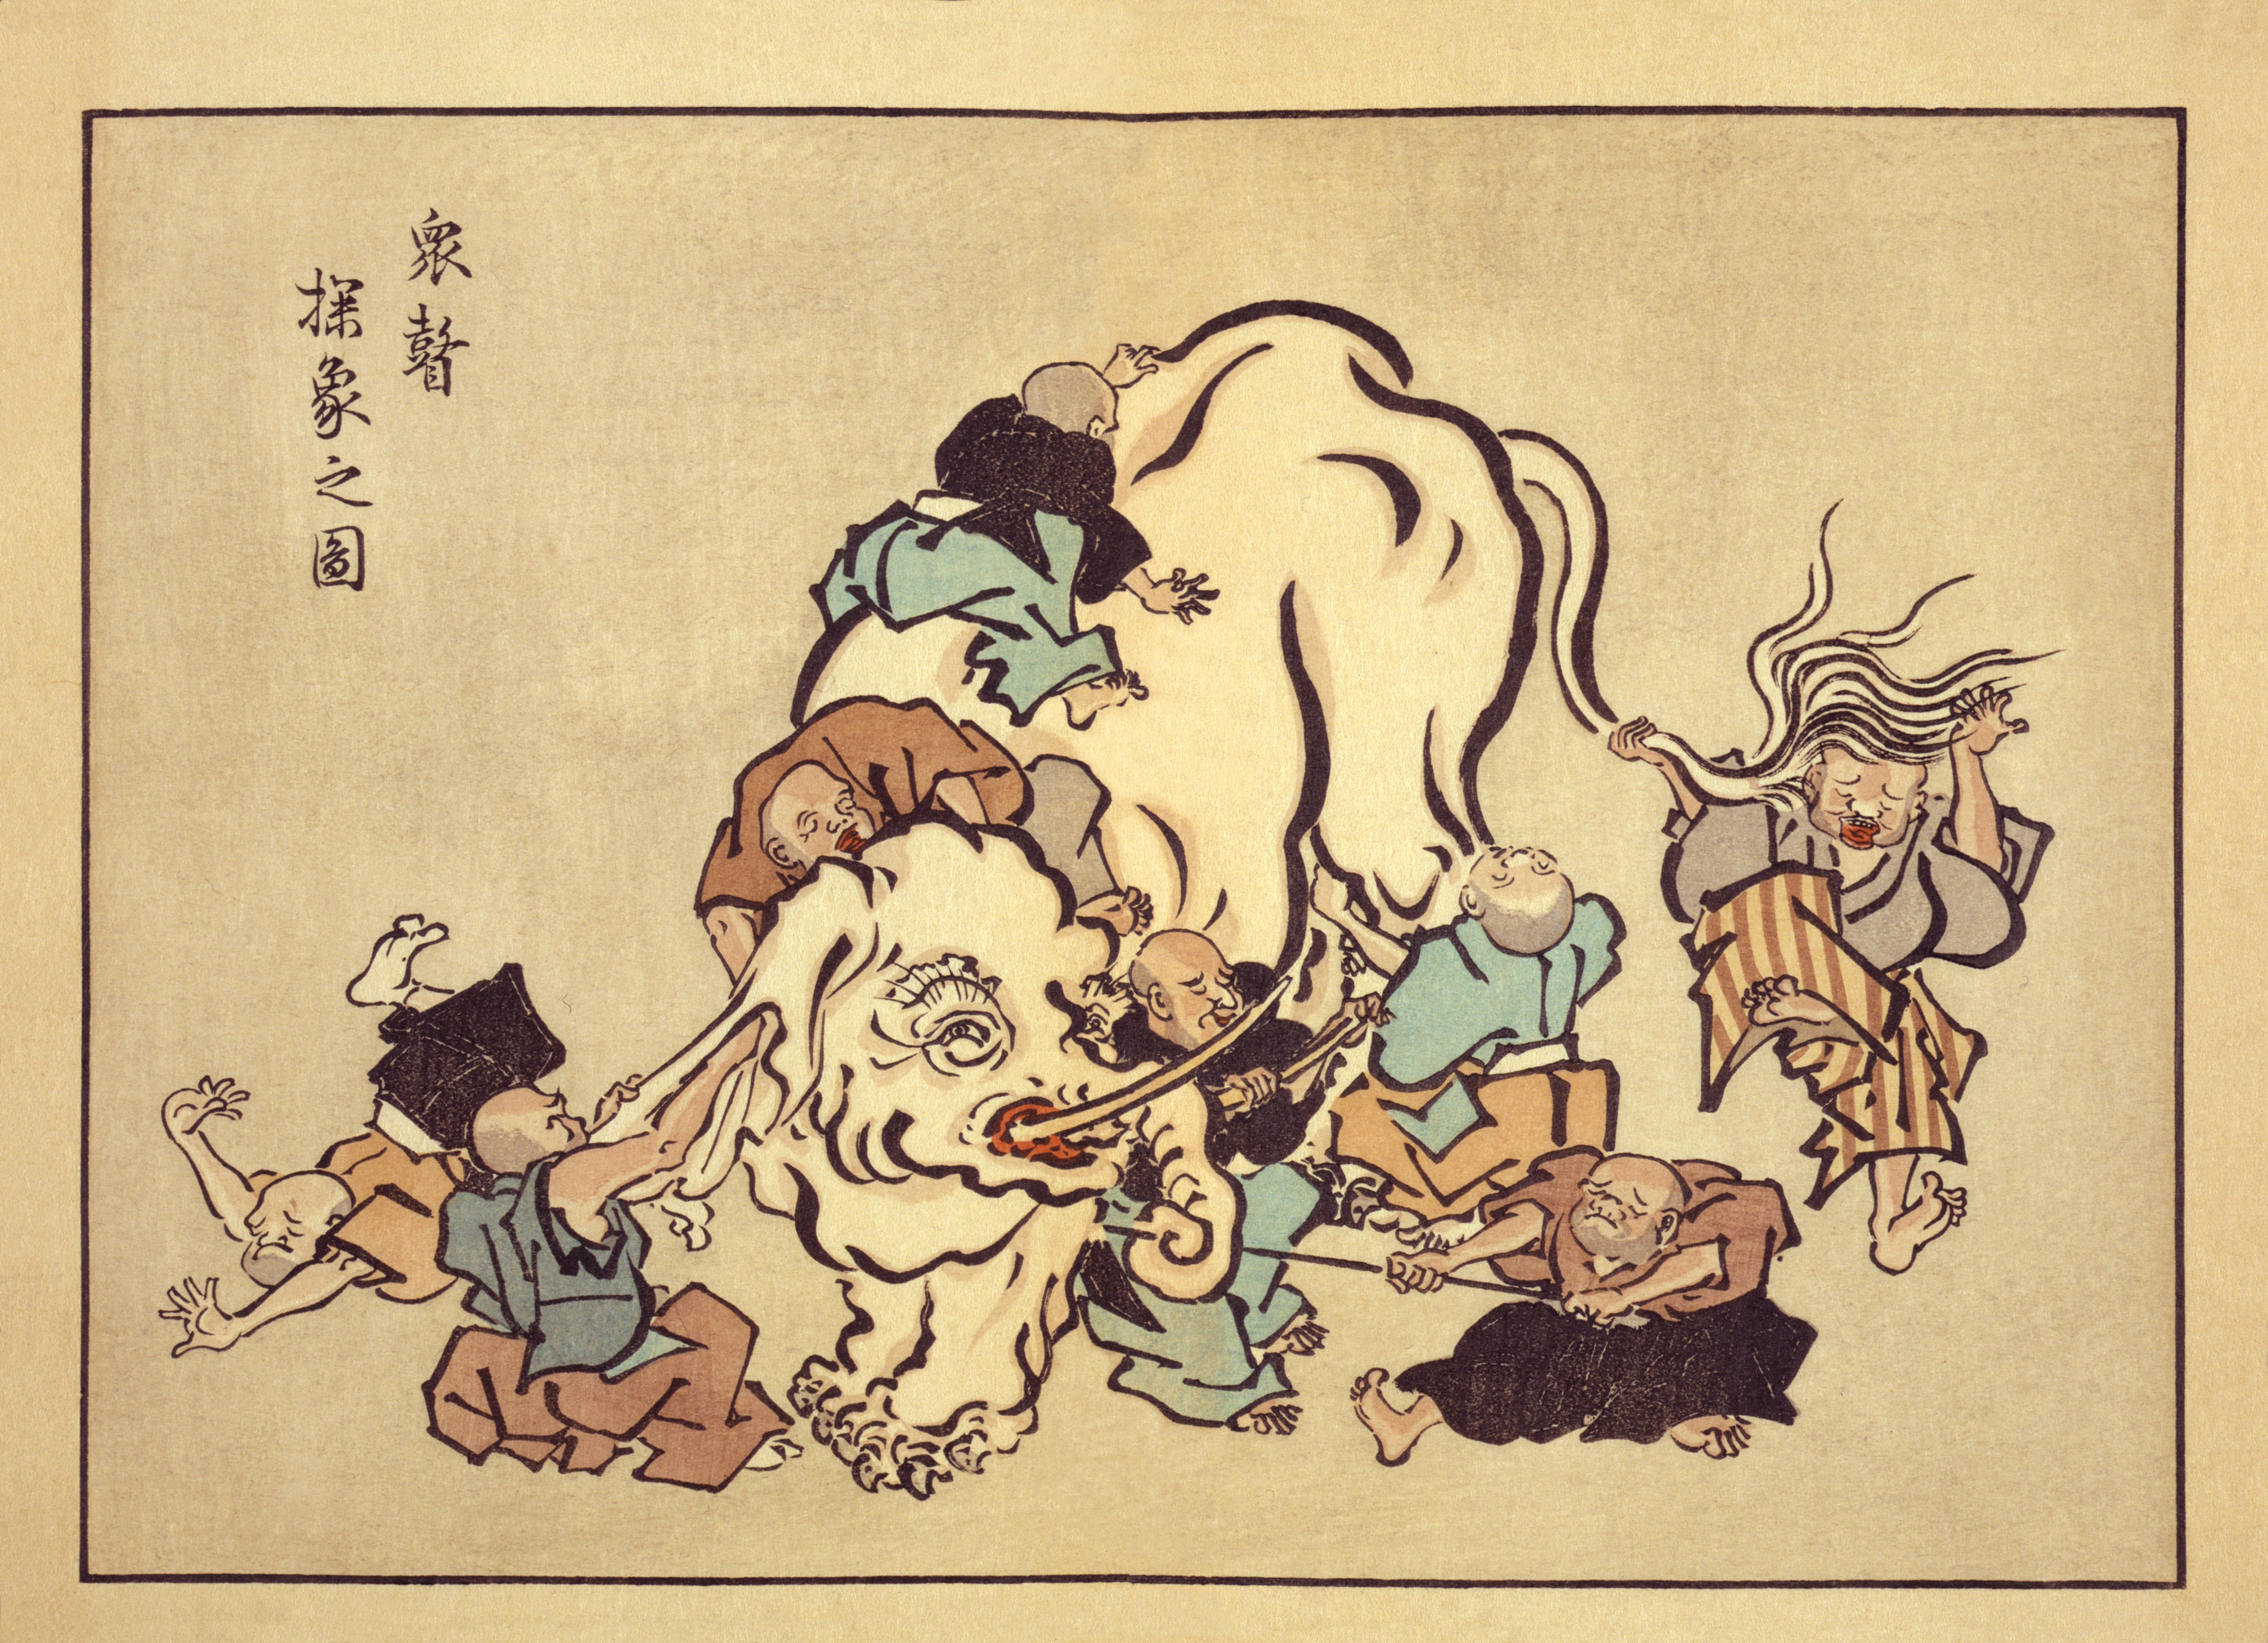
\includegraphics[width=90mm]{assets/images/blind-monks.jpg}
\caption{Blind monks examining the Bitcoin bull\label{fig:blind-monks}}
\end{figure}

Bitcoin is a child of many disciplines. Like blind monks examining an elephant,
everyone who approaches this novel technology does so from a different angle.
And everyone will come to different conclusions about the nature of the beast.

The following lessons are about some of my assumptions which Bitcoin shattered,
and the conclusions I arrived at. Philosophical questions of immutability,
scarcity, locality, and identity are explored in the first four lessons.

\TODO{Lesson List}
% 

Lesson 5 explores how Bitcoin's origin story is not only fascinating but
absolutely essential for a leaderless system. The last two lessons of this
chapter explore the power of free speech and the limits of our individual
knowledge, reflected by the surprising depth of the Bitcoin rabbit hole.

I hope that you will find the world of Bitcoin as educational, fascinating and
entertaining as I did and still do. I invite you to follow the white rabbit and
explore the depths of this rabbit hole. Now hold on to your pocket watch, pop
down, and enjoy the fall.
